% ============================================================================
\section{Theory: the lattice Schwinger model on four qubits}
\label{sec:theory}
% ============================================================================

This section goes from the continuum theory to a lattice, removes the gauge
field and maps the result onto four qubits, following Kogut and Susskind~\cite{kogut1975} and Banks
\emph{et al.}~\cite{banks1976} for the lattice, Hamer \emph{et al.}\ for
eliminating the gauge field~\cite{hamer1997}, and Martinez \emph{et al.}, whose
printed spin Hamiltonian the result matches term by term~\cite{martinez2016}.
Units are natural, $\hbar = c = 1$.

\subsection{The continuum theory}

A Lagrangian density $\mathcal{L}$ is the field version of $T - V$ in
mechanics. The Schwinger model is quantum electrodynamics in one space and one
time dimension~\cite{schwinger1962},
\begin{equation}
  \label{eq:lagrangian}
  \mathcal{L} = \bar\psi\left(i\gamma^\mu D_\mu - m\right)\psi
              - \tfrac14 F_{\mu\nu}F^{\mu\nu},
  \qquad D_\mu = \partial_\mu + i g A_\mu .
\end{equation}
Here $\mu = 0, 1$ labels $t$ and $x$, and repeated indices are summed. The
first term is the matter, a Dirac field $\psi$ of mass $m$ (the $\gamma^\mu$
are fixed $2\times2$ matrices and $\bar\psi = \psi^\dagger\gamma^0$). Through
$D_\mu$ it couples with charge $g$ to the gauge field $A_\mu$, which collects the
scalar and vector potentials. The last term belongs to the field alone, with
$F_{\mu\nu} = \partial_\mu A_\nu - \partial_\nu A_\mu$; in one space dimension
it equals $\tfrac12 E^2$, the electric energy density.

In one spatial dimension the Dirac field needs only two components and there is
no spin: it describes a particle and its antiparticle, each with a single
internal state. With no room for a magnetic field to circulate, only
$E = F_{01}$ remains, and there is no independent propagating photon.

The consequence is confinement. By Gauss's law, $\partial_x E = g\,\psi^\dagger
\psi$, the field between two opposite charges cannot spread out and
stays constant, so the stored energy grows linearly with separation,
$V(r) = \tfrac12 g^2 r$~\cite{coleman1975}. Once that energy exceeds the cost of
a new pair, the vacuum produces one and the string breaks. After a quench, a
start from a state other than the ground state, pairs are produced and
annihilated in real time: the signal whose survival under noise this thesis
measures.

\subsection{Staggered fermions}
\label{sec:staggered}

On a lattice the field lives only on evenly spaced points, the sites, a
distance $a$ apart: a discretisation, like a finite-difference grid, not objects
in nature. The derivative becomes a symmetric difference between neighbouring
sites, whose momentum-space form $(i/a)\sin(pa)$ vanishes at
$p = 0$ and again at $p = \pi/a$, where the field alternates in sign from site
to site. The energy, $\pm\sqrt{\sin^2(pa)/a^2 + m^2}$, is as low there as at
$p = 0$, so the lattice holds a second fermion species, a ``doubler''. Nielsen and Ninomiya proved
that doublers cannot be removed while keeping locality, chiral symmetry (which
keeps left- and right-moving massless fermions separate) and the correct
continuum limit all at once~\cite{nielsen1981}.

Dirac pictured the vacuum as a ``sea'' in which every negative-energy state is
filled; a hole in the sea acts as a particle of opposite charge, the
antiparticle. Kogut and Susskind's staggered fermions give up part of the
chiral symmetry: the two components of $\psi$ sit on alternating sites, so one
single-component fermion per site describes both particle and antiparticle,
and the alternating mode becomes the second component of $\psi$ instead of a
second species~\cite{kogut1975}. The two components enter the mass term with
opposite signs, so a fermion on site $n$ costs $(-1)^n m$
(Eq.~\eqref{eq:H_fermion}). Occupied odd sites lower the energy and play the
sea: in the vacuum they are filled and the even sites empty, so a fermion on an
even site is a particle and an empty odd site an antiparticle. Which is called
the particle is a convention; Martinez \emph{et al.}\ call the even-site
excitation a positron~\cite{martinez2016}, and nothing here depends on the
choice.

The operator $\hat c^\dagger_n$ puts a fermion on site $n$, $\hat c_n$ removes
one, and $\hat c^\dagger_n \hat c_n$ counts them, 0 or 1. Annihilation
operators anticommute, $\hat c_n \hat c_k = -\hat c_k \hat c_n$, which encodes
fermion antisymmetry and, at $n = k$, exclusion; on one site
$\hat c_n\hat c^\dagger_n + \hat c^\dagger_n\hat c_n = 1$. The charge density measures departures from the
vacuum,
\begin{equation}
  \label{eq:charge}
  \hat\rho_n = \hat c^\dagger_n \hat c_n - \frac{1 - (-1)^n}{2},
\end{equation}
zero on every vacuum site, $+1$ on a particle and $-1$ on an antiparticle.

\subsection{Solving Gauss's law}

On the lattice the gauge field lives on the links: link $n$, from site $n$ to
$n+1$, carries an electric field $\hat E_n$ and a phase $\hat U_n$ standing in
for the vector potential. Gauss's law becomes
$\hat E_n - \hat E_{n-1} = \hat\rho_n$, with the field counted in units of
$g$. In three dimensions this only restricts
a field that can circulate; in one it fixes the field. With open boundaries and
no background field, the field left of site~1 vanishes and
\begin{equation}
  \label{eq:gauss}
  \hat E_n = \Lop{n} = \sum_{k \le n} \hat\rho_k .
\end{equation}
Re-phasing each $\hat c_n$ by the link phases to its left, a gauge
transformation like choosing $A_x = 0$ in electromagnetism, removes
$\hat U_n$, and
Eq.~\eqref{eq:gauss} removes $\hat E_n$~\cite{hamer1997,martinez2016}, leaving
fermions alone,
\begin{equation}
  \label{eq:H_fermion}
  \Hop = w\sum_{n=1}^{N-1}\left(\hat c^\dagger_n \hat c_{n+1} + \mathrm{h.c.}\right)
       + m\sum_{n=1}^{N}(-1)^n \hat c^\dagger_n \hat c_n
       + J\sum_{n=1}^{N-1}\Lop{n}^2,
  \qquad w = \frac{1}{2a},\quad J = \frac{g^2 a}{2}.
\end{equation}
Here h.c., the Hermitian conjugate, adds the reverse hop. The hopping strength
$w$ is the $1/2a$ of the symmetric difference, and $J$ comes from the field
energy, $\tfrac12\int E^2\,dx \to \tfrac{a}{2}\sum_n (g\hat E_n)^2$. Hopping
from an occupied odd site to an empty even site creates a particle and an
antiparticle at once, so the first term is the pair-creation operator. Martinez
\emph{et al.}\ write it with a factor $-i$, removed by
$\hat c_n \to i^n \hat c_n$.

This buys $N$ qubits for $N$ sites, with no gauge-field register or
truncation, at the price of locality: $\Lop{n}$ sums the charge on every site
to its left, so $\Lop{n}^2$ couples distant sites.

\subsection{Jordan--Wigner and the spin Hamiltonian}

A site is occupied or empty, so it maps onto a qubit: $|0\rangle$, the
$\Zop{}=+1$ state, is occupied and $|1\rangle$ empty. Fermion operators on
different sites anticommute, however, while operators on different qubits
commute. The
Jordan--Wigner transformation~\cite{jordan1928} supplies the missing signs with
a string of $\Zop{}$ operators on every site to the left, whose sign depends on
the occupations there,
\begin{equation}
  \label{eq:jw}
  \hat c_n = \Bigl(\prod_{k<n}\Zop{k}\Bigr)\sigm{n},
  \qquad \hat c^\dagger_n \hat c_n = \tfrac12\left(1 + \Zop{n}\right),
\end{equation}
with $\sigp{} = |0\rangle\langle 1|$. Between neighbours the strings leave one
$\Zop{}$, so $\hat c^\dagger_n \hat c_{n+1} = -\sigp{n}\sigm{n+1}$. This sign is
real but removable: the relabelling $\hat c_n \to (-1)^n \hat c_n$ flips it
without changing the spectrum, as the code checks.

The filled sea is now $|\mathrm{vac}\rangle = |0101\rangle$, site~1 leftmost,
called the bare vacuum:
the ground state of the mass and electric terms, but not of the full Hamiltonian
once $w \ne 0$. Figure~\ref{fig:states} shows it with the other bitstrings of
zero total charge.

\begin{figure}[t]
  \centering
  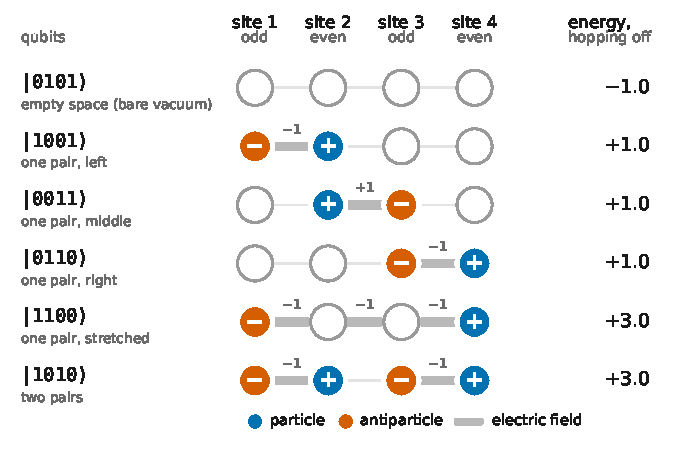
\includegraphics[width=0.72\textwidth]{13_lattice_states.pdf}
  \caption{The six bitstrings of zero total charge, with the charge on each
  site from Eq.~\eqref{eq:charge}, the field on each link from
  Eq.~\eqref{eq:gauss}, and the energy without hopping ($m = 0.5\,w$, $J = w$):
  $m$ per charge plus $J$ per unit of field on each link. Produced by
  \texttt{scripts/13\_lattice\_states.py}.}
  \label{fig:states}
\end{figure} With $\hat\rho_n = \tfrac12[\Zop{n} + (-1)^n]$ the Hamiltonian
becomes a spin chain, up to a constant that vanishes for even $N$,
\begin{equation}
  \label{eq:H}
  \Hop = \frac{m}{2}\sum_{n=1}^{N}(-1)^n \Zop{n}
       + w\sum_{n=1}^{N-1}\left(\sigp{n}\sigm{n+1} + \mathrm{h.c.}\right)
       + J\sum_{n=1}^{N-1}\Lop{n}^2,
  \qquad
  \Lop{n} = \frac12\sum_{k\le n}\left[\Zop{k} + (-1)^k\right].
\end{equation}

Expanded, Eq.~\eqref{eq:H} is a sum of Pauli strings, one Pauli matrix or
identity per qubit, written as words such as \texttt{ZIZI} read from site~1.
The hopping becomes $\tfrac12 w(\Xop{n}\Xop{n+1} + \Yop{n}\Yop{n+1})$. The
electric term couples each pair $k < k' \le N-1$ as
$\tfrac12 J (N - k')\,\Zop{k}\Zop{k'}$, so a neutral pair costs $J$ per link
between its charges: the linear potential on the lattice. Table~\ref{tab:pauli} lists the
fourteen strings at $N = 4$.

\begin{table}[t]
  \centering
  \caption{The $N=4$ Hamiltonian, Eq.~\eqref{eq:H}, as Pauli strings, leftmost
  character on site~1, printed by \texttt{scripts/03\_schwinger\_spectrum.py}.
  The three constructions of Section~\ref{sec:verification} agree exactly at
  these parameters and to \num{9e-16} or better at every other parameter set
  tried.}
  \label{tab:pauli}
  \small
  \begin{tabular}{llll}
    \toprule
    String & Coefficient & String & Coefficient \\
    \midrule
    \texttt{IIII} & $+2J$                      & \texttt{IIXX}, \texttt{IIYY} & $+\tfrac12 w$ \\
    \texttt{IIIZ} & $+\tfrac12 m$              & \texttt{IXXI}, \texttt{IYYI} & $+\tfrac12 w$ \\
    \texttt{IIZI} & $-\tfrac12 m - \tfrac12 J$ & \texttt{XXII}, \texttt{YYII} & $+\tfrac12 w$ \\
    \texttt{IZII} & $+\tfrac12 m - \tfrac12 J$ & \texttt{ZZII}                & $+J$ \\
    \texttt{ZIII} & $-\tfrac12 m - J$          & \texttt{ZIZI}, \texttt{IZZI} & $+\tfrac12 J$ \\
    \bottomrule
  \end{tabular}
\end{table}

\subsection{Parameters}
\label{sec:parameters}

All results use $N = 4$, $J = w$ and $m = 0.5\,w$, those of the main data set
of Martinez \emph{et al.}~\cite{martinez2016}, with time in units of $1/w$.
Since $J/w = (ag)^2$, this is $ag = 1$ and $m/g = 0.25$, a coarse lattice far
from the continuum limit, about which no claim is made.

\subsection{Symmetries that survive as diagnostics}
\label{sec:symmetries}

Gauss's law, $\Lop{n} - \Lop{n-1} - \hat\rho_n = 0$, holds identically in this
encoding (Section~\ref{sec:intro-diagnostic}), so diagnostics must come from
the two exact symmetries below. Both gate-noise models break them, but
logical-frame dephasing respects both (Section~\ref{sec:diagnostics}).

\emph{Total charge.} $\hat Q = \sum_n \hat\rho_n$ commutes with $\Hop$, so a
state stays in its charge sector, the bitstrings with a given $Q$. The bare
vacuum lies in the neutral sector: the six ``physical states'' Martinez
\emph{et al.}\ list~\cite{martinez2016}, those with two occupied sites.

\emph{CP inside the neutral sector.} CP is built from two lattice operations:
$\hat X^{\otimes N}$, which flips every qubit, and the mirror reflection $R$ of
site $n$ to $N+1-n$. Each alone also swaps the roles of odd and even sites,
turning $|0101\rangle$ into $|1010\rangle$, a state of different mean energy,
which an operator commuting with $\Hop$ could not do. In the product
$\mathrm{CP} = R\,\hat X^{\otimes N}$ the two swaps cancel, leaving charge
conjugation (particles exchanged with antiparticles) times parity (the mirror).
It moves each charge to the mirror site with its sign flipped,
$\hat\rho_n \to -\hat\rho_{N+1-n}$, and summing over the sites left of link $n$
gives
\begin{equation}
  \label{eq:cpL}
  \Lop{n} \to \Lop{N-n} - \hat Q ,
\end{equation}
the $-\hat Q$ arising because $\Lop{n}$ counts charge from the left end. The
mass and hopping terms are unchanged by CP in every sector, but the electric
term only when $Q = 0$: otherwise the cross term $-2\hat Q\Lop{N-n}$ survives.
CP therefore commutes with $\Hop$ in the neutral sector only. A neutral
state that CP leaves unchanged up to a phase, called CP-symmetric, therefore has
\begin{equation}
  \label{eq:cp}
  \langle \Lop{n} \rangle = \langle \Lop{N-n} \rangle .
\end{equation}
Neutrality alone is not enough: $|0110\rangle$ is neutral, but its links carry
$(0, 0, -1)$. CP returns the bare vacuum to itself, so every state evolved from
it is CP-symmetric too, and so is the ground state. Every factor of the Trotter
step conserves $\hat Q$ and commutes with CP in the neutral sector, so the
noiseless circuit keeps Eq.~\eqref{eq:cp} exactly at any step size, and a
violation larger than its shot-noise error bar comes from hardware error.

\subsection{Observables}
\label{sec:observables}

The physics observable is the particle density of Martinez
\emph{et al.}~\cite{martinez2016}, the mean number of particles plus
antiparticles per site,
\begin{equation}
  \label{eq:nu}
  \nu(t) = \frac{1}{2N}\sum_{n=1}^{N}\left[1 + (-1)^n\langle\Zop{n}(t)\rangle\right].
\end{equation}
It is zero on the bare vacuum, and at $N = 4$, $\nu = 1/2$ means one pair on
average. For
the ground state the observable is the chiral condensate
$\langle\bar\psi\psi\rangle = (2N)^{-1}\sum_n (-1)^n\langle\Zop{n}\rangle$, the
ground-state value, per site, of the operator that the mass multiplies. Since
$\nu = \tfrac12 + \langle\bar\psi\psi\rangle$, the density and the condensate
are the same operator up to a constant. The mass term is
$mN\bar\psi\psi$, so the Hellmann--Feynman theorem,
$dE_0/dm = \langle\partial\Hop/\partial m\rangle$, gives
$\langle\bar\psi\psi\rangle = N^{-1}\,dE_0/dm$ for the ground state.

The simulation starts in the bare vacuum, where the mass and electric terms are
at their minima, $-mN/2$ and zero. Forming pairs raises both, and since the
total energy is conserved exactly, the hopping term, initially zero, falls by
the same amount. At the first maximum of the density, $t = 0.89$, the mass and
electric terms have gained 0.93 and 0.97 and the hopping term has lost 1.90.
